\sujet{Logarithmic Image Processing (LIP)}
\index{Frameworks!Logarithmic Image Processing}

\begin{note}\textls[-10]{This tutorial aims to study the LIP model, which is a vector space of gray-level images, consistent with the physical laws of Weber and Fechner as well with the visual perception laws.
More particularly, the LIP dynamic expansion, used for image enhancement, will be implemented as well as the Sobel LIP filter for edge detection.}\end{note}


\noindent The different processes will be applied on a mammographic image.
\vspace*{-5pt}
\begin{figure}[htbp]
\begin{center}
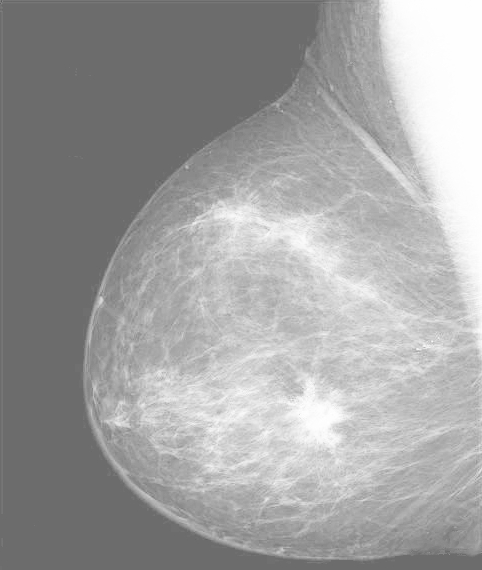
\includegraphics[width=3.7cm]{breast.jpg}
\caption{Breast}
\vspace*{-8pt}
\end{center}
\end{figure}

\vspace*{-14pt}
\section{Introduction}
\vspace*{-6pt}
The LIP model (Logarithmic Image processing) has been introduced in the mid 1980s. It defines a mathematical framework for image processing in a bounded interval.  It is mathematically rigorous and physically justified. For more informations, refer to \cite{Pinoli1987,Jourlin1987,Pinoli1997}. 

An image is represented by its gray-tone function $f$, defined on a spatial domain  $D\subset\R^2$, and with values into $[0,M[$, where $M>0$. For all gray-tone functions $S$ defined on  $D$, a vector space is defined by the operations of addition $\lipplus{}$ and multiplication $\lipfois{}$, and by extension with  the operations of subtraction $\lipmoins{}$ and negation:\vspace*{-10pt}

\begin{align}
 \forall f, g \in S, ~f\lipplus{}g&=f+g-\frac{fg}{M} \\
 \forall f\in S, \forall \lambda\in\R, ~\lambda\lipfois{} f &= M-M\Big(1-\frac{f}{M}\Big)^\lambda \\
 \forall f\in S, ~\lipmoins{} f &= \frac{-Mf}{M-f} \\
 \forall f,g\in S, ~f\lipmoins{}g &= M\frac{f-g}{M-g}
\end{align}

The vector space $S$ of gray-tone functions is algebrically and topologically isomorph to the classical vector space, defined by the isomorphism $\varphi$:\vspace*{-5pt}
\begin{equation}\forall f\in S, ~\varphi(f) = -M \textrm{ln}\Big(1-\frac{f}{M}\Big)
\end{equation}


The inverse isomorphism $\varphi^{-1}$ is then defined by:\vspace*{-5pt}
\begin{equation}f = \varphi^{-1}(\varphi(f)) = M\Big( 1-\textrm{exp}\Big(-\frac{\varphi(f)}{M}\Big)\Big)
\end{equation}


This fundamental isomorphism allows the definition of the following operations on gray-tone functions:
\begin{itemize}
 \item Dot product: $\forall f,g \in S, <f,g>_{\lip{}}=\int\varphi(f)\varphi(g)$
 \item Euclidean norm: $\forall f \in S,\ \Vert f\Vert_{\lip{}} = |\varphi(f)|_\R$, with $|\cdot|_\R$ is the classical absolute value.
\end{itemize}

\vspace*{-12pt}

\section{Elementary LIP operations}
Classically, gray-tones are coded with 8 bits, and thus one can choose $M=256$. Be careful that there might exist sampling issues, and it might be required to considere images in the LIP space with a double precision.

\begin{qbox}
\begin{enumerate}
	\item Implement the elementary LIP operations $\lipplus{}$, $\lipfois{}$ and $\lipmoins{}$.
	\item Test these operators on the image 'breast'.
\end{enumerate}
\end{qbox}

\vspace*{-12pt}

\section{LIP dynamic expansion}
The LIP model enables to define an image transformation that expanses, in an optimal way, the overall dynamic range (gray-tones) while preserving a physical or visual sense.
Let a graytone function denoted $f$ be defined on the spatial support $D\subset\R^2$. Its upper and lower bounds are denoted $\displaystyle f_u=\sup_{x\in D} f(x)$ and $\displaystyle f_l=\inf_{x\in D} f(x)$, with $0<f_l<f_u<M_0$.

The dynamic range of $f$ on $D$ is defined by $R(f)= f_u-f_l$. The LIP scalar multiplication of $f$ by a real number $\lambda>0$ yields to the following dynamic : \begin{equation}
R(\lambda\lipfois{}f) = \lambda\lipfois{}f_u - \lambda\lipfois{}f_l
\end{equation}


It has been shown \cite{Jourlin1995} that there exists an optimal value $\lambda_0(f)$ that maximizes the dynamic range, i.e.: 
\begin{equation}
R(\lambda_0(f)\lipfois{}f)=\max_{\lambda>0}R(\lambda\lipfois{}f).
\end{equation}

\begin{qbox}
\begin{enumerate}
	\item Determine the explicit (analytic) expression of the parameter $\lambda_0(f)$.
	\item Calculate the value of the parameter $\lambda_0(f)$ for the image 'breast'.
	\item Enhance the image and compare the result with the histogram equalization.
\end{enumerate}
\end{qbox}

\begin{mcomment}
\begin{mremark}
Histogram equalization in \matlabregistered{} is performed with the \minline{histeq} function.
\end{mremark}
\end{mcomment}

\begin{pcomment}
\begin{premark}
\textls[-15]{In python, one can use the scikit-image module, and the \pinline{skimage.exposure.equalize_hist} function.}
\end{premark}
\end{pcomment}

\vspace*{-12pt}

\section{LIP edge detection}
\begin{qbox}
\begin{enumerate}
	\item Implement the Sobel filter within the LIP framework.
	\item Compare the results with the classical Sobel filter.
\end{enumerate}
\end{qbox}
